\documentclass[a4paper,14pt]{extarticle}

\usepackage[utf8x]{inputenc}
\usepackage[T1,T2A]{fontenc}
\usepackage[russian]{babel}
\usepackage{hyperref}
\usepackage{indentfirst}
\usepackage{here}
\usepackage{array}
\usepackage{graphicx}
\usepackage{caption}
\usepackage{subcaption}
\usepackage{chngcntr}
\usepackage{amsmath}
\usepackage{amssymb}
\usepackage{amsthm}
\usepackage{pgfplots}
\usepackage{pgfplotstable}
\usepackage[left=2cm,right=2cm,top=2cm,bottom=2cm,bindingoffset=0cm]{geometry}
\usepackage{multicol}
\usepackage{askmaps}
\usepackage{titlesec}
\usepackage{listings}
\usepackage{color}
\usepackage{enumerate}
\usepackage{hhline}
\usepackage{enumitem}
\usepackage{courier}
\usepackage{wrapfig}
\usetikzlibrary{arrows,automata}

\setitemize{itemsep=0em}
\setenumerate{itemsep=0em}

\theoremstyle{definition}

\pgfkeys{/pgf/number format/.cd,1000 sep={\,}}

\definecolor{green}{rgb}{0,0.6,0}
\definecolor{gray}{rgb}{0.5,0.5,0.5}
\definecolor{purple}{rgb}{0.58,0,0.82}

\lstset{
	language=python,
	backgroundcolor=\color{white},   
	commentstyle=\color{green},
	keywordstyle=\color{blue},
	numberstyle=\tiny\color{gray},
	stringstyle=\color{purple},
	basicstyle=\footnotesize\ttfamily,
	breakatwhitespace=false,
	breaklines=true,
	captionpos=b,
	keepspaces=true,
	numbers=left,
	numbersep=5pt,
	showspaces=false,
	showstringspaces=false,
	showtabs=false,
	tabsize=2,
	frame=single,
	inputpath={../code/}
}

\renewcommand{\le}{\ensuremath{\leqslant}}
\renewcommand{\leq}{\ensuremath{\leqslant}}
\renewcommand{\ge}{\ensuremath{\geqslant}}
\renewcommand{\geq}{\ensuremath{\geqslant}}
\renewcommand{\epsilon}{\ensuremath{\varepsilon}}
\renewcommand{\phi}{\ensuremath{\varphi}}
\renewcommand{\thefigure}{\arabic{figure}} 	
\newcommand{\norm}[1]{\left\lVert#1\right\rVert}
\newcommand*\sfrac[2]{{}^{#1}\!/_{#2}}

%\titleformat*{\section}{\large\bfseries} 
\titleformat*{\subsection}{\normalsize\bfseries} 
\titleformat*{\subsubsection}{\normalsize\bfseries} 
\titleformat*{\paragraph}{\normalsize\bfseries} 
\titleformat*{\subparagraph}{\normalsize\bfseries} 

\counterwithin{figure}{section}
\counterwithin{equation}{section}
\counterwithin{table}{section}
\newcommand{\sign}[1][5cm]{\makebox[#1]{\hrulefill}}
\graphicspath{{../pics/}}
\captionsetup{justification=centering,margin=1cm}
\setlength\parindent{5ex}
\def\arraystretch{1.3}
\def\tabcolsep{12pt}
%\titlelabel{\thetitle.\quad}

\DeclareMathOperator*{\argmin}{argmin}
\DeclareMathOperator*{\argmax}{argmax}

\begin{document}

\begin{titlepage}
\begin{center}
	\textbf{Санкт-Петербургский Политехнический Университет \\Петра Великого}\\[0.3cm]
	\small Институт компьютерных наук и технологий \\[0.3cm]
	\small Кафедра компьютерных систем и программных технологий\\[4cm]
	
	\textbf{ОТЧЕТ}\\ \textbf{по расчетному заданию}\\[0.5cm]
	\textbf{<<Построение моделей>>}\\[0.1cm]
	\textbf{Системный анализ и принятие решений}\\[8.0cm]
\end{center}

\begin{flushright}
	\begin{minipage}{0.4\textwidth}
		\begin{flushleft}
			\small \textbf{Работу выполнил студент}\\[3mm]
			\small группа 33501/4 \hspace*{6mm} Дьячков В.В.\\[5mm]
			
			\small \textbf{Преподаватель}\\[5mm]
		 	\small \sign[3cm] \hspace*{5mm} Сабонис С.С.\\[0.5cm]
		\end{flushleft}
	\end{minipage}
\end{flushright}

\vfill

\begin{center}
	\small Санкт-Петербург\\
	\small \the\year
\end{center}
\end{titlepage}

\addtocounter{page}{1}

\tableofcontents
\listoffigures
\newpage

\section{Техническое задание}

\paragraph{Вариант 32.} 
Сравнить средние времена пребывания и средние времена ожидания для разных систем в зависимости от интенсивности потока заявок. Построить соответствующие графики. Какая система лучше (при каких интенсивностях первая система лучше, при каких – вторая)? 
	
\section{Исходные данные}

\begin{figure}[H]
	\begin{subfigure}{\textwidth}
		\centering
		\begin{tikzpicture}[start chain=going right,>=latex,node distance=0pt]
			\node[rectangle split, minimum height=2cm, draw, rectangle split horizontal, on chain] (wa) {
				$\infty$
				\nodepart{two} $\circ$
				\nodepart{three} $\circ$
				\nodepart{four} $\circ$
			};
			\draw[<-] (wa.west) -- +(-1.2,0) node[left] {$\lambda$};
			\draw[->] (wa.east) -- +(60:2.1) coordinate (B1);
			\draw[->] (wa.east) -- +(30:1.2) coordinate (B2);
			\draw[->] (wa.east) -- +(-30:1.2) coordinate (B3);
			\draw[->] (wa.east) -- +(-60:2.1) coordinate (B4);
			\node[draw,rectangle,on chain,minimum size=1cm] at (B1) (se1) {$\mu$};
			\node[draw,rectangle,on chain,minimum size=1cm] at (B2) (se2) {$\mu$};
			\node[draw,rectangle,on chain,minimum size=1cm] at (B3) (se3) {$\mu$};
			\node[draw,rectangle,on chain,minimum size=1cm] at (B4) (se4) {$\mu$};
			\draw[-] (se1.east) --+(-60:2.1) coordinate (C1);
			\draw[-] (se2.east) --+(-30:1.2) coordinate (C2);
			\draw[-] (se3.east) --+(30:1.2) coordinate (C3);
			\draw[-] (se4.east) --+(60:2.1) coordinate (C4);
			\draw[->] (C2)--+(0:1.2)node[right] (C4) {};
		\end{tikzpicture}
		\caption{}
	\end{subfigure}
	\begin{subfigure}{\textwidth}
		\centering
		\begin{tikzpicture}[start chain=going right,>=latex,node distance=0pt]
			\node[rectangle split, minimum height=2cm, draw, rectangle split horizontal, on chain] (queue1) {
				$\infty$
				\nodepart{two} $\circ$
				\nodepart{three} $\circ$
				\nodepart{four} $\circ$
			};
			\draw[<-] (queue1.west) -- +(-1.2,0) node[left] {$\lambda$};
			\draw[->] (queue1.east) -- +(60:2.1) coordinate (B1);
			\draw[->] (queue1.east) -- +(30:1.2) coordinate (B2);
			\draw[->] (queue1.east) -- +(-30:1.2) coordinate (B3);
			\draw[->] (queue1.east) -- +(-60:2.1) coordinate (B4);
			\node[draw,rectangle,on chain,minimum size=1cm] at (B1) (chan1) {$2\mu$};
			\node[draw,rectangle,on chain,minimum size=1cm] at (B2) (chan2) {$2\mu$};
			\node[draw,rectangle,on chain,minimum size=1cm] at (B3) (chan3) {$2\mu$};
			\node[draw,rectangle,on chain,minimum size=1cm] at (B4) (chan4) {$2\mu$};
			\draw[-] (chan1.east) --+(-60:2.1) coordinate (C1);
			\draw[-] (chan2.east) --+(-30:1.2) coordinate (C2);
			\draw[-] (chan3.east) --+(30:1.2) coordinate (C3);
			\draw[-] (chan4.east) --+(60:2.1) coordinate (C4);
			\draw[->] (C2)--+(0:1.2)node[right] (C5) {};
			\node[rectangle split, minimum height=2cm, draw, rectangle split horizontal, on chain] at (C5.west) (queue2) {
				$\infty$
				\nodepart{two} $\circ$
				\nodepart{three} $\circ$
				\nodepart{four} $\circ$
			};
			\draw[->] (queue2.east) -- +(60:2.1) coordinate (D1);
			\draw[->] (queue2.east) -- +(30:1.2) coordinate (D2);
			\draw[->] (queue2.east) -- +(-30:1.2) coordinate (D3);
			\draw[->] (queue2.east) -- +(-60:2.1) coordinate (D4);
			\node[draw,rectangle,on chain,minimum size=1cm] at (D1) (chan5) {$2\mu$};
			\node[draw,rectangle,on chain,minimum size=1cm] at (D2) (chan6) {$2\mu$};
			\node[draw,rectangle,on chain,minimum size=1cm] at (D3) (chan7) {$2\mu$};
			\node[draw,rectangle,on chain,minimum size=1cm] at (D4) (chan8) {$2\mu$};
			\draw[-] (chan5.east) --+(-60:2.1) coordinate (E1);
			\draw[-] (chan6.east) --+(-30:1.2) coordinate (E2);
			\draw[-] (chan7.east) --+(30:1.2) coordinate (E3);
			\draw[-] (chan8.east) --+(60:2.1) coordinate (E4);
			\draw[->] (E4)--+(0:1.2)node[right] (E5) {};
		\end{tikzpicture}
		\caption{}
	\end{subfigure}
	\caption{Структуры сравниваемых сетей}
	\label{fig:structure}
\end{figure}

\section{Сравнение систем массового обслуживания}

\subsection{Однофазная система массового обслуживания}
\label{sec:onephase}

На рис. \ref{fig:state_graph} приведен граф состояний системы $M/M/4$.

\begin{figure}[H]
	\centering
	\begin{tikzpicture}[->,>=stealth',shorten >=1pt,auto,node distance=2.4cm,semithick]
		\tikzstyle{every state}=[fill=white,draw=black,text=black]
		
		\node[state] (0) {$0$};
		\node[state] (1) [right of=0] {$1$};
		\node[state] (2) [right of=1] {$2$};
		\node[state] (3) [right of=2] {$3$};
		\node[state] (4) [right of=3] {$4$};
		\node[state,draw=white] (5) [right of=4] {\Large$\dots$};
		
		\path 
		(0) edge [bend left] node {$\lambda$} (1)
		(1) edge [bend left] node {$\mu$} (0)
		(1) edge [bend left] node {$\lambda$} (2)
		(2) edge [bend left] node {$2\mu$} (1)
		(2) edge [bend left] node {$\lambda$} (3)
		(3) edge [bend left] node {$3\mu$} (2)
		(3) edge [bend left] node {$\lambda$} (4)
		(4) edge [bend left] node {$4\mu$} (3)
		(4) edge [bend left] node {$\lambda$} (5)
		(5) edge [bend left] node {$4\mu$} (4);
	\end{tikzpicture}
	\caption{Граф состояний}
	\label{fig:state_graph}
\end{figure}

\noindent Показатели системы $M/M/K$ рассчитываются по формулам:
\begin{itemize}
	\item Коэффициенты загруженности системы:
		\begin{displaymath}
			\rho = \dfrac{\lambda}{\mu}, \quad \rho_c = \dfrac{\lambda}{K \cdot \mu}
		\end{displaymath}
	\item Вероятность нахождения системы в состоянии $i$:
		\begin{displaymath}
			P_i = 
			\begin{cases}
				\left( 1 + \sum \limits_{j=1}^{K} \dfrac{\rho^j}{j!} + \dfrac{\rho^{K+1}}{K! \cdot (K - \rho)} \right)^{-1} &\text{ если } i = 0 \\[15pt]
				\dfrac{\rho^i \cdot P_0}{i!} &\text{ если } i \leq K \text{ и } i \neq 0 \\[15pt]
				\dfrac{\rho^i \cdot P_0}{K! \cdot K^{i-K}} &\text{ если } i > K
			\end{cases}
		\end{displaymath}
		
	\item Средняя длина очереди:
		\begin{displaymath}
			\overline{n_\text{о}} = \dfrac{\rho^{K+1} \cdot P_0}{K \cdot (1 - \rho_c)^2 \cdot K!}
		\end{displaymath}
		
	\item Среднее число занятых каналов:
		\begin{displaymath}
			\overline{K_\text{з}} = \rho
		\end{displaymath}
		
	\item Среднее число клиентов в системе:
		\begin{displaymath}
			\overline{j} = \overline{n_\text{о}} + \overline{K_\text{з}}
		\end{displaymath}
		
	\item Среднее время ожидания:
		\begin{displaymath}
			t_\text{ож} = \dfrac{\overline{n_\text{о}}}{\lambda} = \dfrac{\overline{n_\text{о}}}{\rho \cdot \mu}
		\end{displaymath}
		
	\item Среднее время обслуживания:
		\begin{displaymath}
			t_\text{c} = \dfrac{\overline{j}}{\lambda} = \dfrac{\overline{j}}{\rho \cdot \mu} = t_\text{ож} + \dfrac{1}{\mu}
		\end{displaymath}
\end{itemize}

\newpage

\subsection{Двухфазная система массового обслуживания}

Система состоит из двух последовательных фаз с бесконечными очередями, следовательно можно рассмотреть по-отдельности первую и вторую фазы, а потом сложить их показатели. Так как эти фазы одинаковы, то достаточно найти показатели для одной фазы и умножить на $2$. Характеристики фазы рассчитываются по тем же формулам, что и показатели для однофазной системы массового обслуживания в пункте \ref{sec:onephase}. На рис. \ref{fig:state_graph_2} приведен граф состояний двухфазной системы массового обслуживания.

\begin{figure}[H]
	\centering
	\begin{tikzpicture}[->,>=stealth',shorten >=1pt,auto,node distance=2.4cm,semithick]
	\tikzstyle{every state}=[fill=white,draw=black,text=black]
	
	\node[state] (0) {$0$};
	\node[state] (1) [right of=0] {$1$};
	\node[state] (2) [right of=1] {$2$};
	\node[state,draw=white] (3) [right of=2] {\Large$\dots$};
	\node[state] (8) [right of=3] {$8$};
	\node[state] (9) [right of=8] {$9$};
	\node[state,draw=white] (10) [right of=9] {\Large$\dots$};
	
	\path 
	(0) edge [bend left] node {$\lambda$} (1)
	(1) edge [bend left] node {$2\mu$} (0)
	(1) edge [bend left] node {$\lambda$} (2)
	(2) edge [bend left] node {$4\mu$} (1)
	(2) edge [bend left] node {$\lambda$} (3)
	(3) edge [bend left] node {$6\mu$} (2)
	(3) edge [bend left] node {$\lambda$} (4)
	(8) edge [bend left] node {$16\mu$} (3)
	(8) edge [bend left] node {$\lambda$} (9)
	(9) edge [bend left] node {$16\mu$} (8)
	(9) edge [bend left] node {$\lambda$} (10)
	(10) edge [bend left] node {$16\mu$} (9);
	\end{tikzpicture}
	\caption{Граф состояний}
	\label{fig:state_graph_2}
\end{figure}

\subsection{Сравнение систем}

Для начала рассмотрим зависимость среднего времени пребывания в сети $t_\text{с}$ от интенсивности обслуживания $\mu$ и интенсивности потока заявок $\lambda$. На рис. \ref{fig:tgrid} изображена данная зависимость для однофазной системы.

\begin{figure}[H]
	\vspace{-0.5cm}
	\centering
	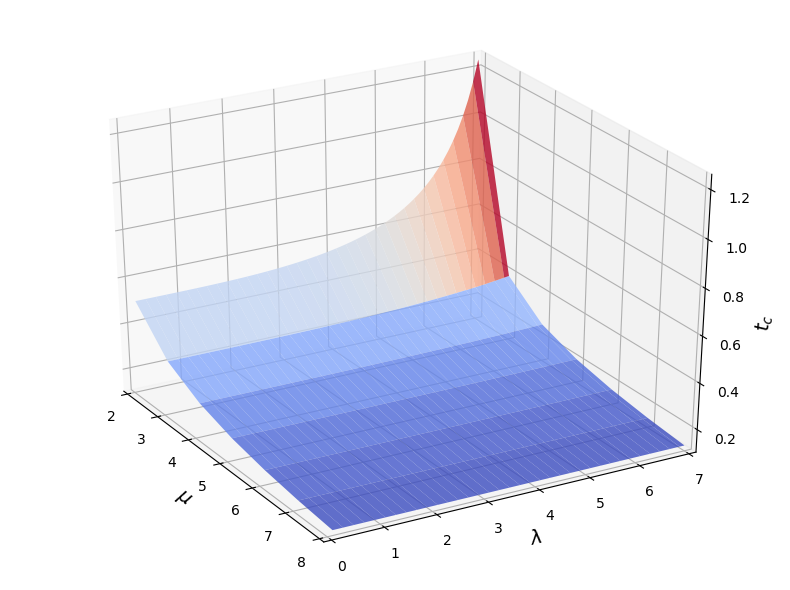
\includegraphics[width=0.95\textwidth]{tgrid}
	\caption{Зависимость $t_\text{с}$ от $\mu$ и $\lambda$ для однофазной системы}
	\label{fig:tgrid}
	\vspace{-0.5cm}
\end{figure}

\newpage

Зафиксируем $\mu = 5$ и рассмотрим зависимость среднего времени ожидания $t_\text{ож}$ от интенсивности потока заявок $\lambda$. На рис. \ref{fig:tw} изображена данная зависимость для обеих систем.
\begin{figure}[H]
	\vspace{-0.4cm}
	\centering
	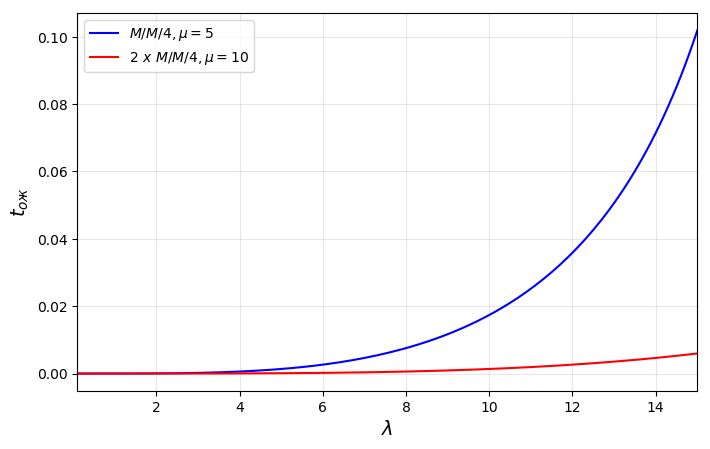
\includegraphics[width=0.85\textwidth]{tw}
	\caption{Зависимость $t_\text{ож}$ от $\lambda$}
	\label{fig:tw}
	\vspace{-0.3cm}
\end{figure}

Рассмотрим зависимость среднего времени пребывания в системе $t_\text{с}$ от интенсивности потока заявок $\lambda$ при $\mu = 5$. На рис. \ref{fig:t} изображена данная зависимость для обеих систем.
\begin{figure}[H]
	\vspace{-0.4cm}
	\centering
	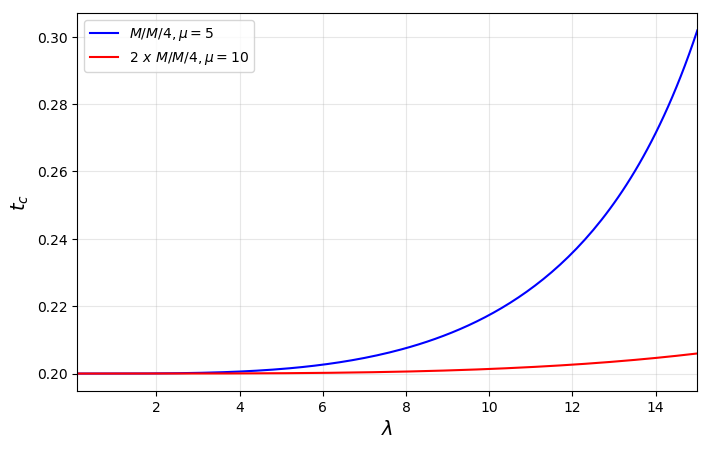
\includegraphics[width=0.85\textwidth]{t}
	\caption{Зависимость $t_\text{с}$ от $\lambda$}
	\label{fig:t}
	\vspace{-0.3cm}
\end{figure}

Из графиков можно сделать вывод, что среднее время ожидания и обслуживания в двухфазной системе растет медленнее, чем в однофазной, следовательно по данным параметрам она является предпочтительной.

\end{document}